\chapter{Referencial Teórico}

Para gerar os gráficos, fazer análises, determinar o valor e o método de correlação, fazer as tabelas e os mapas coropléticos, escolheu-se a linguagem de programação \textbf{Python}.

Foram usadas as bibliotecas \textbf{Pandas} para a análise exploratória de dados, \textbf{GeoPandas} para os mapa coropléticos, \textbf{Matplotlib} e \textbf{Seaborn} para a geração  de gráficos.Usou-s a biblioteca \textbf{great_tables} para gerar as tabelas em formato \textbf{PNG}. Para a geração dos mapas foram usados os arquivos do tipo \textbf{SHP} projeto \textbf{Natural Earth Data} para os mapa \textit{mundi} e da malha municipal do Instituto Brasileiro de Geografia e Estatística (IBGE). O tamanho das figuras é padronizado, conforme expresso na figura \ref{fig:tabela_tamanho_figuras}. Porém, tamanhos divergentes podem ser adotados, caso seja necessário.

\begin{figure}[H]
    \centering
    \caption{Tamanho das figuras}
    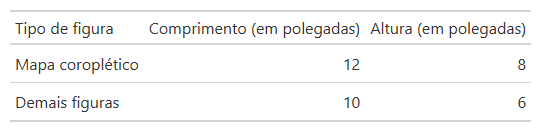
\includegraphics[width=1\linewidth]{figuras/tabela_tamanho_figuras}
    \label{fig:tabela_tamanho_figuras}
    \footnotesize{Fonte: elaboração própria.}
\end{figure}

Além dos argumentos anteriores, o coeficiente de correlação escolhido para todas as análises foi o de \textbf{Spearman}. \cite{hauke2011comparison} explica que o \textbf{coeficiente de correlação de Spearman} é uma estatística de postos não paramétrica (sem distribuição) proposta como uma medida da força da associação entre duas variáveis. É uma medida de uma associação monótona, usada quando a distribuição de dados torna o coeficiente de correlação de Pearson indesejável ou enganoso. 

Além disso, \cite{hauke2011comparison} esclarece que o \textbf{coeficiente de correlação de Spearman} não é uma medida da relação linear entre duas variáveis. Ele avalia quão bem uma função monotônica arbitrária pode descrever a relação entre duas variáveis, sem fazer quaisquer suposições sobre a distribuição de frequência das variáveis.

Ao contrário do \textbf{coeficiente de correlação de Pearson}, segundo \cite{hauke2011comparison}, ele não requer a suposição de que a relação entre as variáveis seja linear, nem requer que as variáveis sejam medidas em escalas intervalares; pode ser usado para variáveis medidas no nível ordinal.

Como forma de poder julgar qualquer valor de coeficiente de correlação encontrado, adotou-se a ideia de \cite{ali2022spearman}, presente na figura \ref{fig:tabela_faixas_correlacao}.

\begin{figure}[H]
    \centering
    \caption{Faixas do coeficiente de correlação}
    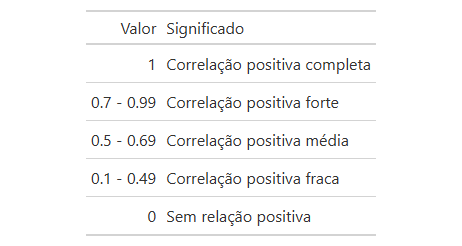
\includegraphics[width=1\linewidth]{figuras/tabela_faixas_correlacao}
    \label{fig:tabela_faixas_correlacao}
    \footnotesize{Fonte: elaboração própria baseada em \cite{ali2022spearman}.}
\end{figure}

Para qualquer coeficiente de correlação presente neste trabalho, adotar-se-ão os critérios presentes na figura \ref{fig:tabela_faixas_correlacao} para determinar a existência ou não de correlação entre as variáveis comparadas.